\documentclass[12pt]{scrartcl}%{article} % Beginn der LaTeX-Datei
\usepackage{scrlayer-scrpage}
\pagestyle{scrheadings}
\usepackage{tabularx}
\usepackage{lastpage}
\usepackage{amsmath,amssymb}
\usepackage[yyyymmdd,hhmmss]{datetime}
\usepackage{graphicx}

\usepackage[english]{babel}
\usepackage[T1]{fontenc}
\usepackage{lmodern}
\usepackage{csvsimple}
\usepackage[ansinew]{inputenc}  % Unix
  % \usepackage[ansinew]{inputenc}  % Windows
  % \usepackage[applemac]{inputenc} % Mac
  
\usepackage[a4paper, left=2cm, right=2cm, top=3.5cm]{geometry}
\setlength{\headsep}{0.5cm}

\ihead{\includegraphics[scale=0.18]{Zahner_Logo.pdf}}

\usepackage{lmodern}
\cfoot{Page \thepage}

\usepackage[thmmarks,amsmath,hyperref,noconfig]{ntheorem}
  
\usepackage[colorlinks,
pdfpagelabels,
pdfstartview = FitH,
bookmarksopen = true,
bookmarksnumbered = true,
linkcolor = black,
plainpages = false,
hypertexnames = false,
citecolor = black] {hyperref}  


\usepackage{color}
\definecolor{white}{rgb}{1,1,1}
\definecolor{darkred}{rgb}{0.3,0,0}
\definecolor{darkgreen}{rgb}{0,0.3,0}
\definecolor{darkblue}{rgb}{0,0,0.3}
\definecolor{pink}{rgb}{0.78,0.09,0.51}
\definecolor{purple}{rgb}{0.28,0.24,0.55}
\definecolor{orange}{rgb}{1,0.6,0.0}
\definecolor{grey}{rgb}{0.4,0.4,0.4}


\DeclareMathOperator{\GL}{GL}
\newcommand{\N}{\mathbb{N}}
\newcommand{\Z}{\mathbb{Z}}
\newcommand{\Q}{\mathbb{Q}}
\newcommand{\R}{\mathbb{R}}
\newcommand{\C}{\mathbb{C}}
\newcommand{\cP}{{\mathcal P}} 

\begin{document}
\vspace*{30mm}
\begin{center}
\title{Capacitor Test Report}
\textbf{{\huge Capacitor Test Report}}
\end{center}
\vspace*{40mm}


\section{Informations}
\vspace{5mm}
\begin{center}
\begin{tabularx}{0.8\textwidth}{| X | X |}
\hline
&\\
\textbf{Test object name}: & C1234\\
&\\
\hline
&\\
\textbf{Date of test}: & \today\\
&\\
\hline
&\\
\textbf{Time of test}: & \currenttime\\
&\\
\hline
&\\
\textbf{Calculated capacity}: & 2.388 mF\\
&\\
\hline
\end{tabularx}
\end{center}
\newpage

\section{CV}
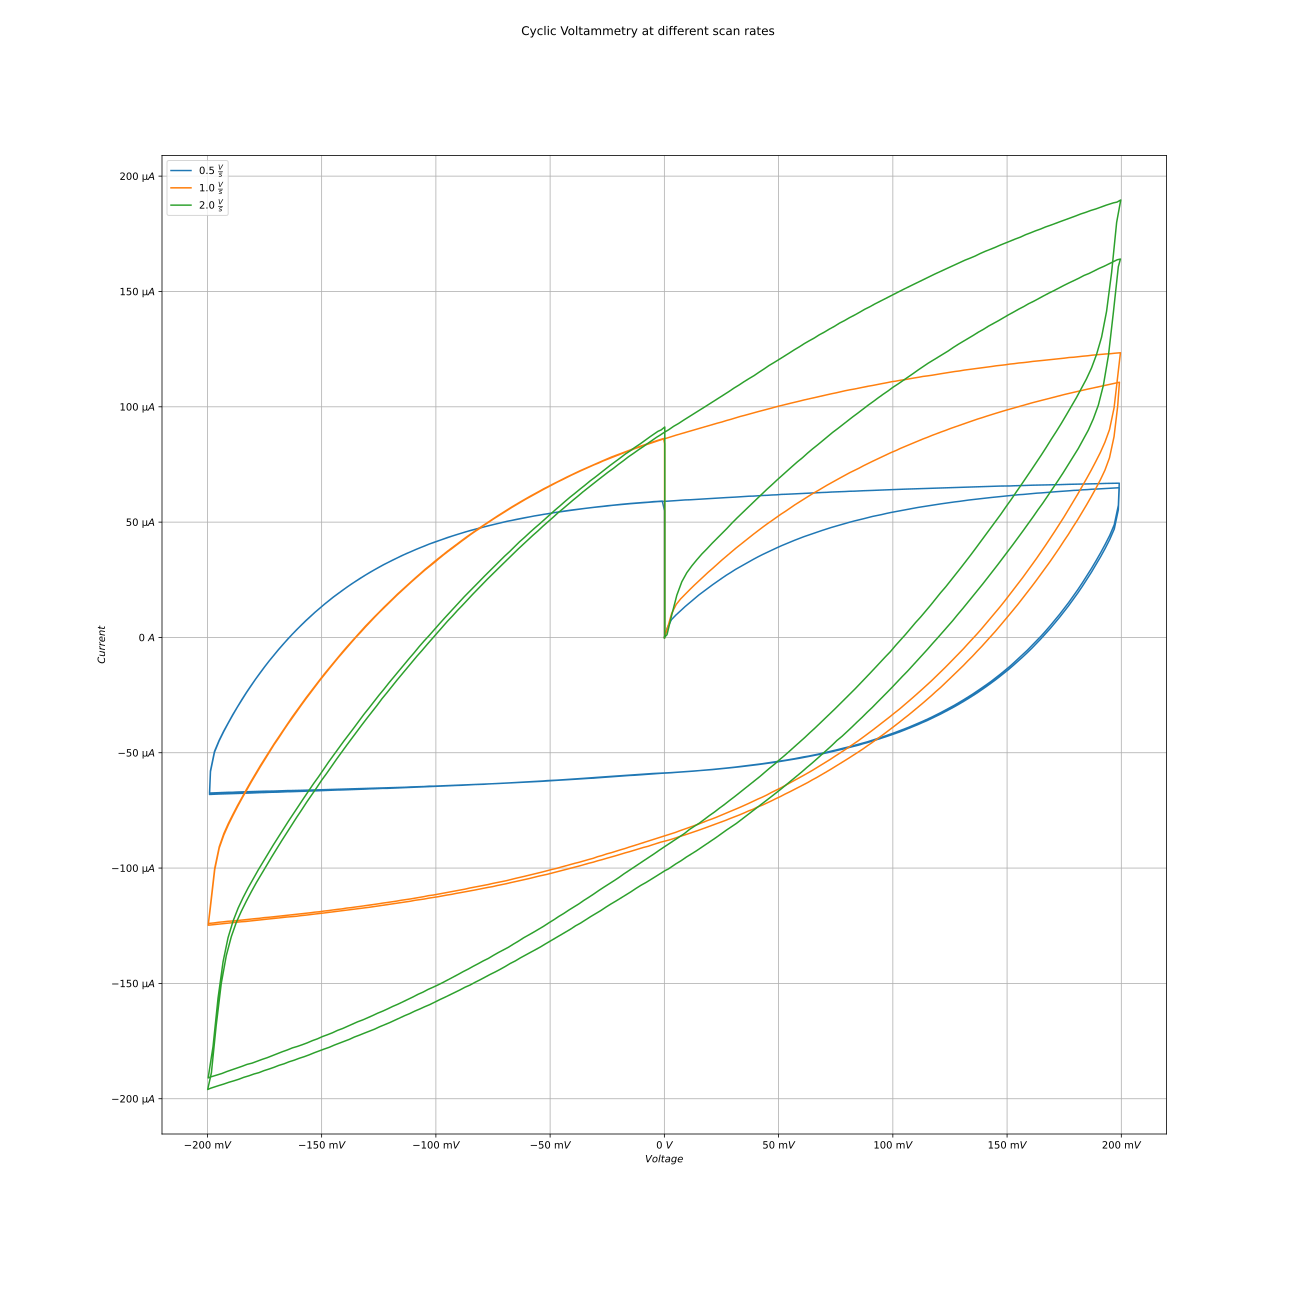
\includegraphics[width=1\textwidth]{ CV.pdf }

\begin{center}
\begin{math}
Capacity = \dfrac{I}{\frac{dV}{dt}} = \dfrac{\dfrac{598.904 \mu A - (-595.283 \mu A)}{2}}{0.25 \frac{V}{s}} = 2.388 mF
\end{math}
\end{center}

\newpage

\section{EIS}
\includegraphics[width=1\textwidth]{ EIS.pdf }

\begin{center}
\begin{tabular}{c|c|c}
\bfseries Frequency $[Hz]$ &  \bfseries |Impedance| $[\Omega]$ & \bfseries Phase [\textdegree]
\csvreader[head to column names, /csv/separator=semicolon]{ EIS.csv }{}
{\\\hline \Frequency & \Impedance & \Phase}
\end{tabular}
\end{center}


\end{document}